\chapter{Le développement de \textit{GreenT}}
Comme nous l'avons montré dans le chapitre \ref{chapPb}, l'entreprise a besoin d'un nouvel outil aidant aux tests d'intégration : \textit{GreenT}. Nous allons donc voir le développement et la conception de cet plateforme de tests.
	\section{Fonctionnement général de la plateforme}
	Lorsque je suis arrivé sur le projet, une partie de la conception était déjà réalisé, le fonctionnement général de la plateforme. Cette conception permet de répondre aux attentes du problème, tout en permettant le maximum d'évolutions facilement.
	
	\subsection{Le fichier Walkthrough}\label{wt}
		Le fichier Walkthrough est un fichier qui sera fournis par la personne en charge des tests, c'est un fichier au format Excel qui contient les informations de chacune des variables à tester. Il contient ainsi un très grand nombre de colonnes, bien que seul une partie des colonnes nous intéresse, certaines colonnes ont été fournis par le fournisseur du plugin, d'autres colonnes sont ajoutés dans le seul but que GreenT génère les tests automatiques. Voici les colonnes intéressantes : 

		\begin{description} 
			\item[Nom de la variable] Le nom de la variable testé : il existe un nom court et un nom long.
			\item[Informations aidant à la conversion des données] Certains devices tel que le débugger ne fonctionne qu'avec des valeurs Hexadécimales. \'A' la charge de GreenT de convertir ces données vers des valeurs physiques exploitables par le testeur
			\item[Nécessité d'un test automatique] un GreenTTest ne sera généré que si la colonne vaut \textit{Yes}.
			\item[Statut du test] Nous éditerons cette colonne afin de reporter le statut du test.
			\item[Precondition (cf section \ref{stim})] Contient un scénario d'initialisation du workbench : tension de départ, lancement du débugger, ...
			\item[Scénario de stimulation (cf section \ref{stim})] Contient un ou plusieurs scénarios de stimulations
			\item[ExpectedBehavior (cf section \ref{expectedBehavior})] Contient une expression évaluant les variables ayant été enregistrés durant la stimulation : GreenT devra vérifier que cette expression est vérifiée à toute instant de la stimulation.
			\item[variable à enregistrer (cf section \ref{expectedBehavior})] Contient les variables devant être enregistrer durant un scénario, en plus des variables présentes dans l'expected behavior.
			\item[Alias locaux (cf section \ref{alias})] Ce sont des alias déclaré uniquement pour le test courant.
			\item[Informations du test (cf section \ref{report})] Plusieurs colonnes tel que la sévérité, le responsable du test, les commentaires, \ldots
		\end{description}

		\begin{figure}[H]
			\centering
			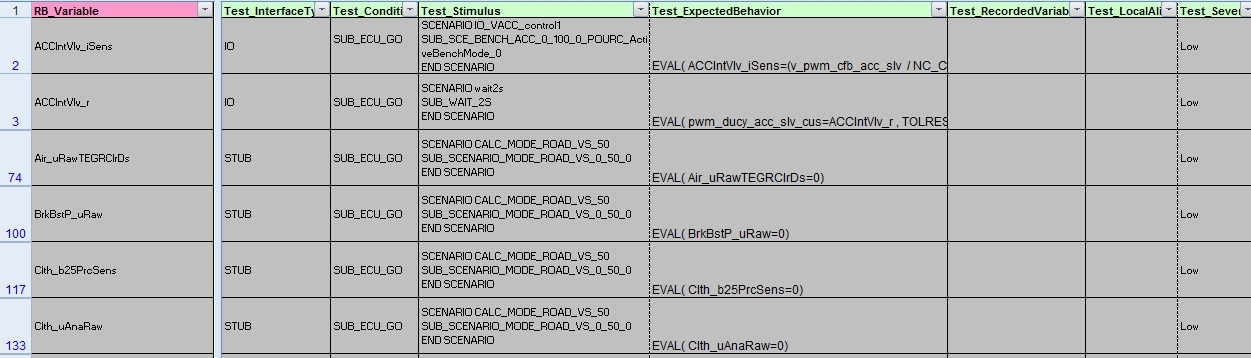
\includegraphics[width=18.5cm]{contents/images/walkthrough.png}
			\caption{Aperçu d'un fichier Walkthrough}
		\end{figure}

	\subsection{Fonctionnalités principales}
	Le développement de GreenT va inclure un certains nombre de fonctionnalités attendu par le client et indispensable à son fonctionnement. D'autres fonctionnalités pourront apparaître plus tard, ainsi les fonctionnalités développées pourront être adaptés.

	L'interaction entre les différents modules de GreenT son schématisés figure \ref{fig:generalDig}

	\subsubsection{Parsing et Génération}\label{generation}
	Le but premier de la plateforme est d'effectuer des tests automatiques, il est ainsi indispensable d'avoir un système d'automatisation.

	Pour cela, nous allons avoir un parser : il analysera un certain type de fichier\footnote{Nous ne commencerons qu'avec le Walkthrough pour débuter, mais dans le futur nous pourrions avoir des fichiers XML, des bases de données, \ldots} et en retirera pour chaque test, le scénario de pré condition, les différents scénarios de stimulations, leurs expectedBehavior, les données qui devront être enregistrés ainsi que les différentes données du test\footnote{Responsable du test, sévérité, commentaires, nom de la variable, \ldots}.

	Une fois toutes ces données acquises, il les transmettra à un générateur qui sera en charge d'écrire les fichiers Java de chaque test, tous seront organisés dans un dossier temporaire avec un dossier par test. Le TestManager pourra ensuite traiter ces données.

	\subsubsection{Résolution des alias}\label{alias}
		Les devices ont des fonctionnements différents pour leurs valeurs internes, le Hil par exemple utilise des adresses de base de données, alors que le debugger fonctionne avec des valeurs Hexa permettant d'accéder directement à des cases RAM.

		Il est donc indispensable de fournir au client une approche permettant de masquer ces différences, et le risque d'erreur en écrivant une adresse, pour cela nous avons pensés un système d'alias : un alias possède un nom qui permet de le lier à une valeur sur le device, le client n'aura ensuite plus qu'à travailler avec des noms clairs et explicites.

		Il y a deux types d'alias : ceux qui sont accessible en écriture, et ceux accessibles en lecture, on pourra donc effectuer des actions différentes en fonction du type d'alias.

	\subsubsection{Stimulation} \label{stim}
		Un test possèdera tout d'abord un scénario de pré condition : celui-ci est nécessaire afin d'initialiser les devices, en initialisant des valeurs, démarrant le débugger, etc\ldots Ceci afin que les résultats des tests soit cohérents.

		Celui-ci possédera également un certain nombre de scénarios de stimulations. Ceux-ci sont des scénarios destinés à effectuer des actions pour mettre le contrôleur en condition, afin de vérifier que le fonctionnement est bien celui attendu. Durant les scénarios de stimulations, des variables sont enregistrés, c'est une fois les stimulations exécutés que l'on peut vérifier que tout s'est passé correctement.

	\subsubsection{Les traces et leurs évaluations}\label{expectedBehavior}
	Lorsqu'un scénario de stimulation s'exécutent, un certain nombre de variables doivent être enregistrés : ces variables sont stockés sous la forme d'une trace au format CSV, qui pourra plus tard être représenté sous forme de courbe. 

	Une fois que la trace est complète, il est nécessaire de l'évaluer : le spécifieur à fournis une expected behavior détaillant dans quel cas le test est correct, ainsi cette expression va être transformé en arbre logique afin de l'évaluer à tout instant T de la trace. Une fonctionnalité de couverture de tests sera fournis afin de s'assurer qu'un test de sévérité \textit{High} est correctement spécifié.

	\subsubsection{TestManager}\label{testManager}
	Le TestManager est le chef d'orchestre de GreenT, il a donc un certain nombre de responsabilités. 

	Il va d'abord organiser les différents tests en un concept que nous avons appelés Bundle : Afin de limiter le temps d'exécution qui atteindra plusieurs dizaines d'heures, il est intéressant de regrouper les tests possédant les mêmes scénarios de stimulations et les mêmes pré conditions : seuls leur expectedBehavior change, mais celles-ci pourront donc être évalués sur la même Trace.

	Une fois les tests organisés en Bundle, il va les compiler et les données à un WorkbenchManager : toujours pour une raison d'optimisation, il sera intéressant de pouvoir exécuter les enregistrements sur plusieurs bancs simultanément, pour cela le TestManager sera capable de savoir quels bancs peuvent être utilisés et pourra distribuer ses bundles en fonction. 

	Chaque WorkbenchManager sera en charge d'exécuter le code généré plus tôt et dialoguera en réseau avec son banc, une fois l'exécution terminée, il obtiendra une trace qui pourra être évaluée.

	Afin d'être le plus souple possible, il existera plusieurs modes d'exécution du TestManager : 
	\begin{description}
		\item[Check only] Essaye de parser les différents fichiers, et vérifie que ceux-ci ne comporte aucune erreur de grammaire, d'alias introuvable, d'écriture sur un alias en lecture seule etc...
		\item[Parse and generate jar tests] Parse les fichiers et génère des jars exécutables pour chacun des tests
		\item[Parse and genere bundles] Parse les fichiers et génère des jars exécutables répartis en bundle
		\item[Parse and execute] Parse les fichiers, génère les jars pour les bundles et les exécute : c'est le mode << classique >>.
		\item[Restart test execution] Redémarre une exécution qui se serait mal terminée.
	\end{description}
	\subsubsection{Production de rapport détaillé}\label{report}
	La plateforme aura en charge la production d'un rapport détaillé pour chaque test. Ce rapport contiendra un certain nombre d'informations, et permettra au testeur de comprendre pourquoi le test n'est pas passé. Voici les informations que contiendra ce rapport : 

	\begin{itemize}
		\item Nom du test, de la variable à tester
		\item Nom du responsable du test
		\item Sévérité du test
		\item Pourcentage de branches de l'expectedBehavior renvoyant faux\footnote{Test << Rouge >>}, n'ayant pas pu être testé\footnote{Test << Gris >>} et étant correct\footnote{Test Vert}
		\item Le testeur aura à sa disposition les expressions concernés par un résultat Rouge ou Gris.
		\item Les colonnes utiles du Walkthrough
	\end{itemize}

	Le format du rapport détaillé n'a pas encore été définis, mais cela pourrait être des fichiers textes, avec pour évolution une possibilité de le faire sous format Web avec affichage des courbes de trace par exemple.

	\subsubsection{Mise à jour du Walkthrough}
	Une fois un test exécuté, un résultat sera mis dans le fichier Excel, en fonction de la sévérité du test. En effet, un test \textit{High} ne devra comporter aucune branche non testée contrairement à un test \textit{Low} par exemple.
	\vfill ~\vfill
	
	\subsubsection{Schéma de fonctionnement global}
		\begin{figure}[H]
			\centering
			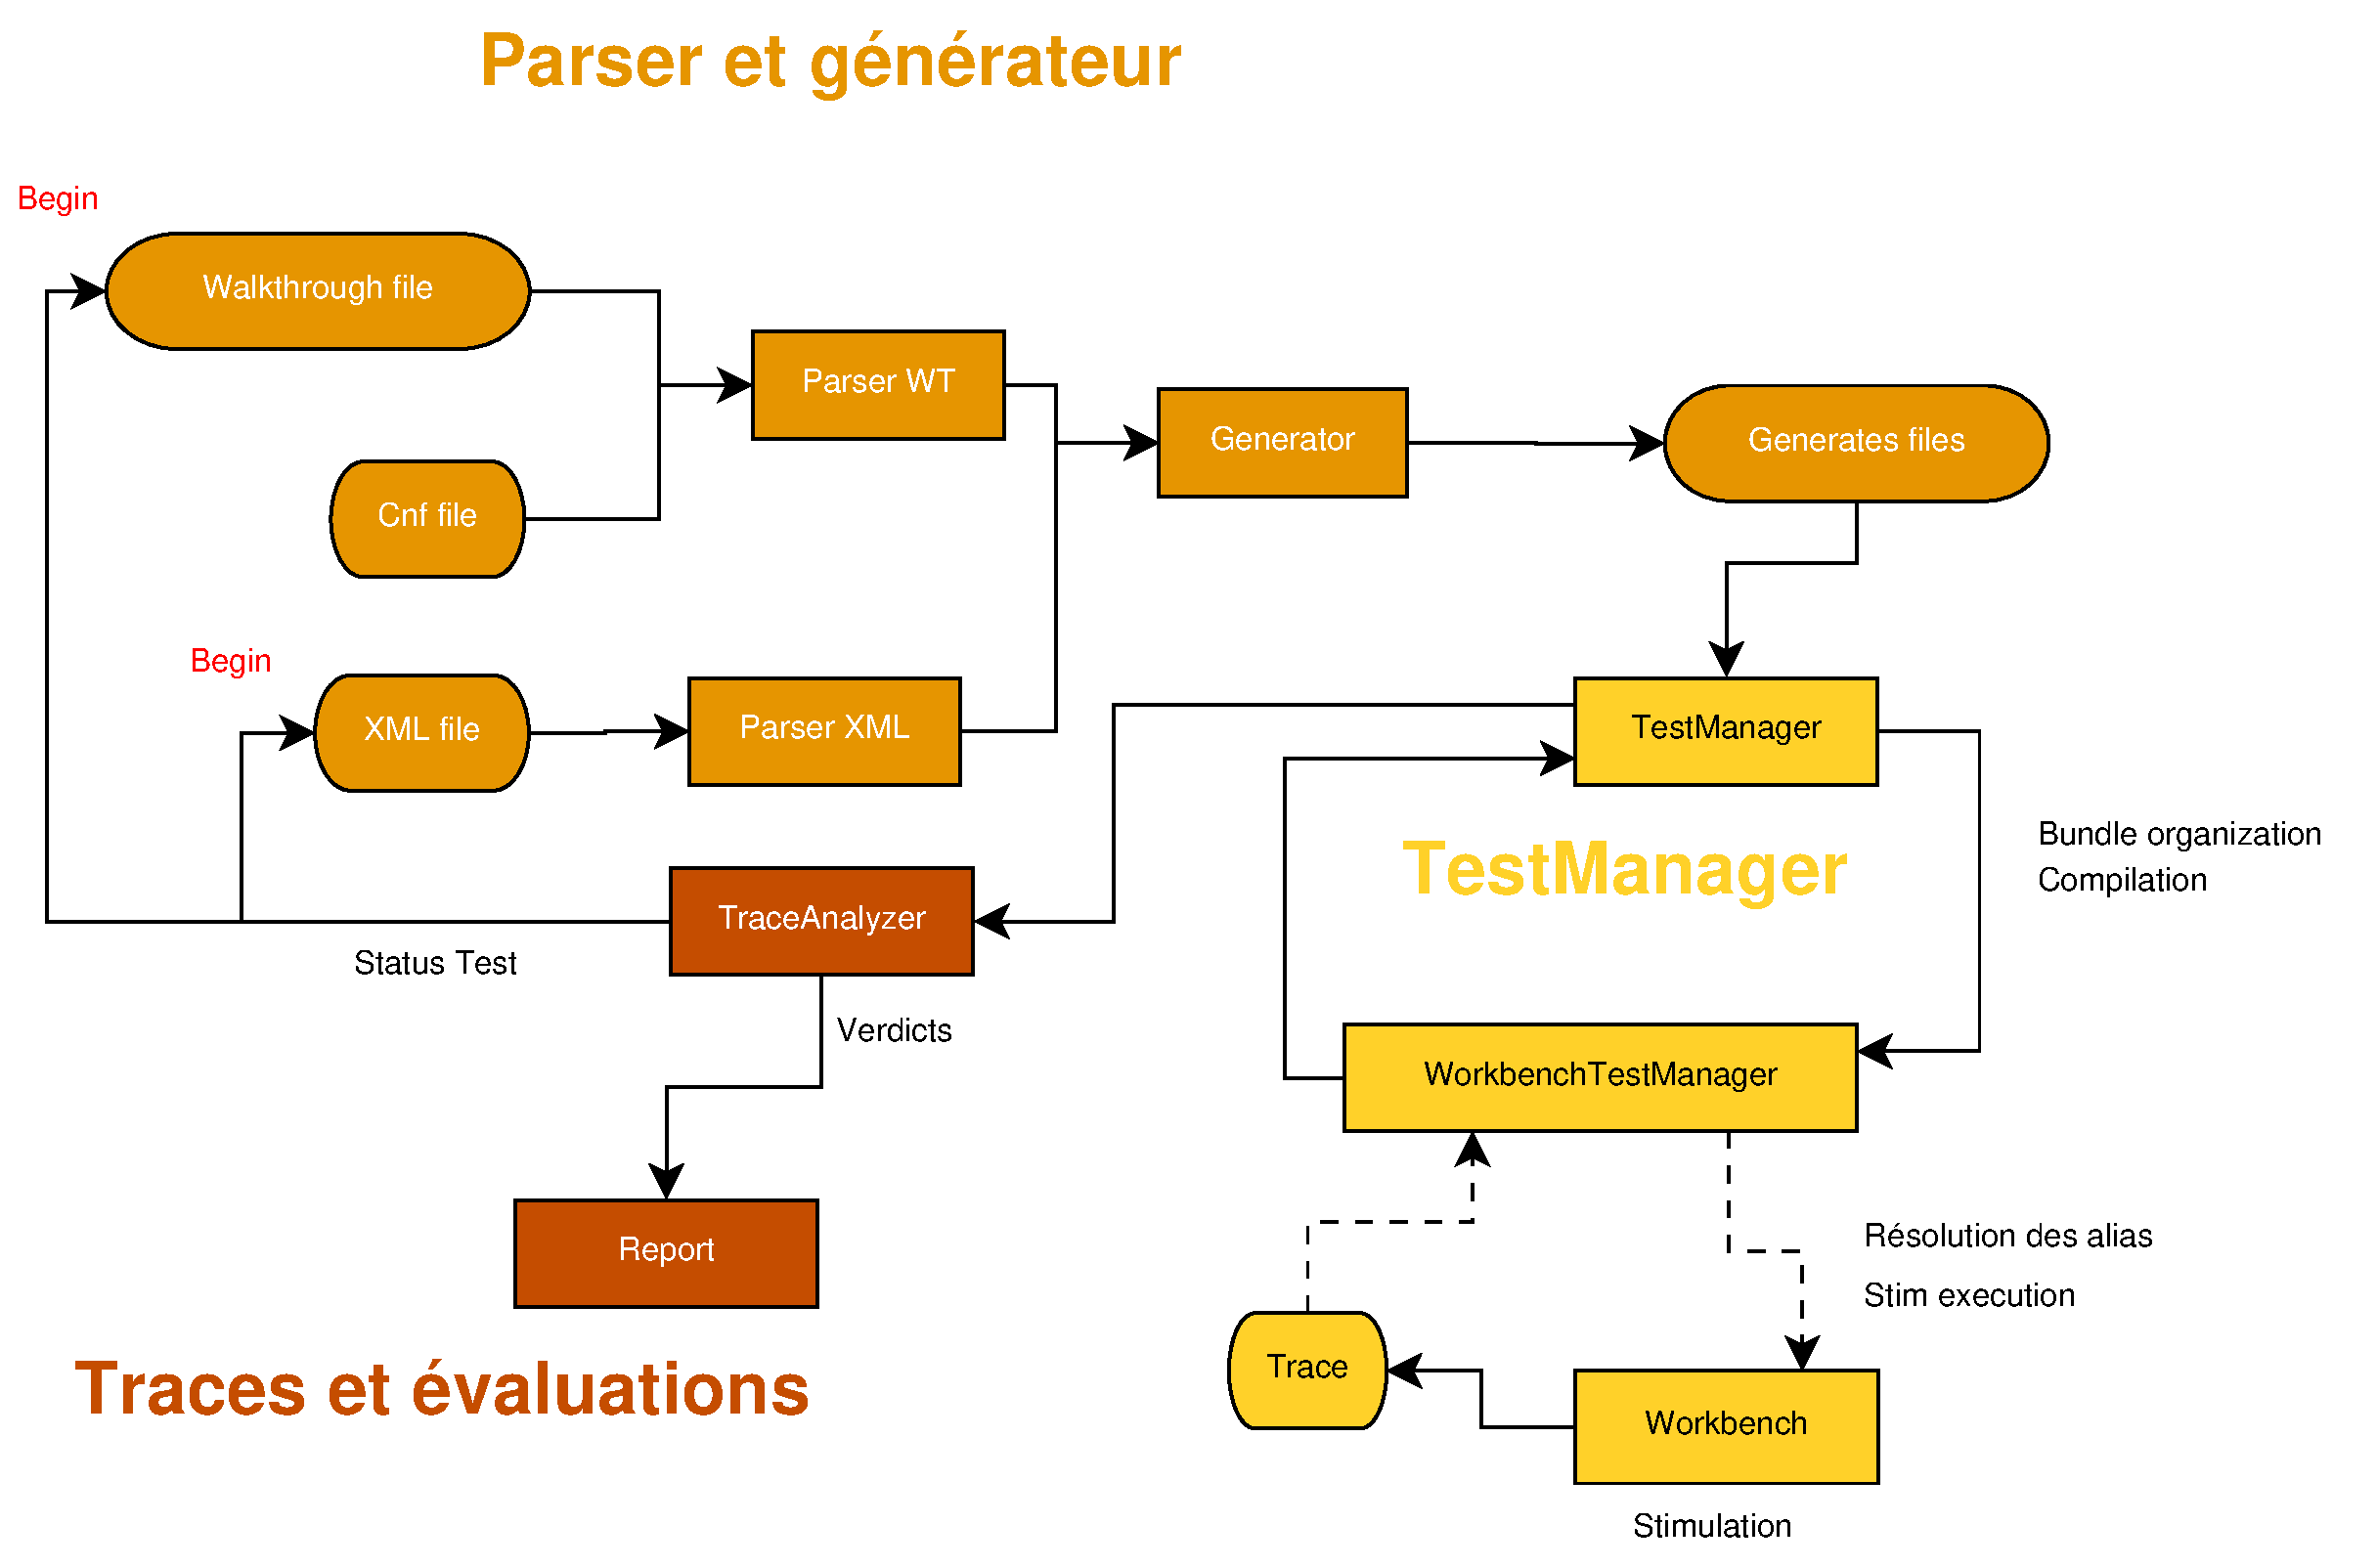
\includegraphics[width=18.5cm]{contents/images/generalDiag.eps}
			\caption{Fonctionnement général du parser GreenT}
			\label{fig:generalDig}
		\end{figure}
		Dans ce schéma nous pouvons voir les différents modules détaillés précédemment : un type de parser prend en entrée un fichier, qu'il analyse, génère les fichiers Java, les donnes au TestManager, qui les organise en Bundle, les compiles, donne les binaires au WorkbenchTestManager, qui dialogue directement avec le banc, une fois le bundle exécuté, celui-ci retourne la trace. Il ne reste plus qu'a l'analyser et prononcer un verdict.\\
		Dans des objets ovales sont représentés des fichiers, les carrés représentent des modules de la plateforme et les flèches en pointillés un transfert réseau.

	Pour ma part, je me suis occupé de la partie du Parser, du générateur, et j'ai aidé à la conception du système d'évaluation et d'analyses des traces.
	\vfill~\vfill
	\section{Ma participation au développement}
	\subsection{Les tableaux callibrables}
	% TODO
	\subsection{Le patch des calibrations}
	% TODO
% 	\section{Le parser}\label{sectionParser}
% 	Avant mon arrivée, le client et l'équipe avait conçus une grammaire de langage permettant de spécifier le fonctionnement du test, ainsi afin d'effectuer un scénario de stimulation où une ExpectedBehavior il faut respecter une syntaxe précise, dans le cas contraire une exception est levée.
% 	\vfill~\vfill

% 	\subsection{La grammaire}
% 	\subsubsection{Les scénarios de stimulations}
% 	Un precondstim peut contenir des affectations, des \textit{check} et des actions débugger : 
% 	\begin{description}
% 		\item[Affectation] Une affectation s'effectue de la façon suivante : \texttt{Alias = valeur}, l'alias \texttt{Alias} sera possédera ensuite la valeur \texttt{valeur}.
% 		\item[Check] Cette action permet de vérifier qu'un alias possède bien la valeur espéré, à une tolérance prêt. Dans le cas contraire le bundle ne pourra pas être exécuté et une exception sera levée. Cela s'effectue ainsi : \texttt{CHECK(Alias = Valeur, TOLRES(tolerance))}, la tolerance étant facultative.
% 		\item[Actions débugger] Il est actuellement possible d'effectuer deux actions : démarrer le debugger, ou l'arrêter : \texttt{T32\_GO} et 
% 		\texttt{T32\_CPU\_STOP}.
% 	\end{description}

% 	Les scénarios de stimulations quant-à eux ont le même fonctionnement, la seule différence est qu'ils doivent être encadrés des balises \texttt{BEGIN SCENARIO nomScenario} et \texttt{END SCENARIO}.

% 	\subsubsection{Le fichier cnf}
% 	Comme nous l'avons expliqué, les tests sont spécifiés dans le fichier Walkthrough qui est au format Excel, étant donné la difficulté d'éditer de longs texte dans la même cellule, il parait important de mettre les scénarios de stimulations dans un autre fichier : c'est l'utilité du fichier cf, celui-ci contiendra des groupes d'actions à effectuer spécifiés par un nom\footnote{Cela pourrai s'approcher du fonctionnement de sous-programmes} : le fichier Excel pourra ainsi ne contenir que le nom du groupe d'action, et de la place sera économisée dans celui-ci.

% 	La syntaxe du fichier est assez simple :
% \begin{lstlisting}[caption=Exemple de fichier cnf, language=C]
% // Section for group of parameters
% SECTION SUB
% 	SUB_ECU_GO : {
% 		HIL_VB = 13;
%  		HIL_KEY = 1;
% 		CHECK(HIL_KEY_OUT = 1);
% 		T32_GO;
% 	}

% 	SUB_ECU_OFF : {
% 		T32_CPU_STOP;
%  		HIL_KEY = 0;
% 		HIL_VB = 0;
% 	}

% 	SUB_SCENARIO_VS_0_50_0 : {
% 		HIL_VS = 0;
% 		CHECK(HIL_VS_OUT = 0,  TOLRES(1)) ;
% 		HIL_VS = 0;
% 		CHECK(HIL_VS_OUT = 50,  TOLPER(1)) ;
% 		HIL_VS = 0;
% 		CHECK(HIL_VS_OUT = 0, TOLRES(1));
% 	}

% END SUB
% \end{lstlisting}
% \begin{remarque}
% Il y a une différence sémantique entre \texttt{TOLRES} et \texttt{TOLPER} : \texttt{TOLRES} est une tolérance en terme de valeur, alors que \texttt{TOLPER} est une tolérance en pourcentage.
% \end{remarque}
% Un simple appel à \texttt{SUB\_ECU\_GO} dans le fichier Excel fera les actions nécessaires. Cette approche permet de gagner de la place comme indiquée, mais elle permet aussi de factoriser les tests !

% 	\subsubsection{Les expected Behavior}
% Comme expliqué précédemment, les Expected Behavior sont des expressions permettant d'évaluer une trace, celles-ci ont une syntaxe proche d'un langage algorithmique : 
% \begin{lstlisting}[caption=Exemple d'expected Behavior, language=Algo]
% if tco > c1 then 
% 	EVAL(lv_cfa = 1)
% else
% 	if(tco < c2) then 
% 		EVAL(lv_cfa = 0)
% 	else           
% 		EVAL(lv_cfa = PRE(lv_cfa))
% 	endif
% endif
% \end{lstlisting}
% La grammaire est donc récursive, il est possible d'effectuer plusieurs Eval à la suite : ceux-ci doivent être séparés par un retour chariot.

% Le mot clé \texttt{PRE} permet de récupérer la valeur précédente de la variable en paramètre, ainsi l'instruction \texttt{lv\_cfa = PRE(lv\_cfa)} permet de vérifier que la variable n'a pas changé.
% \subsubsection{Les alias locaux}
% La dernière grammaire est celle des alias locaux : les alias déclarés uniquement pour le test courant : un certain nombre d'informations est nécessaire : le nom de l'alias, l'adresse, et les informations permettant de convertir celui-ci en valeur physique.

% \begin{lstlisting}[caption=Exemple de définition d'alias local, language=Algo]
% Alias_name = @HEXA;tailleOctet[8000...7FFFH]
% \end{lstlisting}
% L'alias aura une valeur hexadécimale, une taille en nombre d'octet, ainsi qu'une valeur de début et une valeur de fin afin de savoir les limites de définition de cette variable.

% \subsubsection{Variables à enregistrer}
% Il est possible de fournir des variables à enregistrer en plus de celle des expected behavior : cela permet d'avoir le contexte d'exécution, et de mieux comprendre la raison de l'échec d'un test. La définition de ces alias est très simple, ceux-ci doivent simplement être séparés par des virgules.

% \begin{lstlisting}[caption=Exemple de définition d'alias à enregistrer, language=Algo]
% FlSys_stFlLvl, C_FlSys_stFlLvl, LV_REQ_ES_AAS, LV_AAS_ACT
% \end{lstlisting}

% 	\subsection{Implémentation du parser}
% 		\subsubsection{La grammaire : utilisation de Antlr}
% 		\begin{wrapfigure}{r}{3cm}
% 			
\includegraphics[width=3cm]{contents/images/antlr.jpg}
% 		\end{wrapfigure}
% 		J'étais en charge d'écrire le parser spécifié dans la section \ref{sectionParser}. Comme nous l'avons vu, celui-ci intègre beaucoup de grammaires différentes, et celle des expected behavior assez complexe. \\
% 		Une solution à été choisis afin d'optimiser au maximum le temps de développement et de limiter les erreurs : utilisation de Antlr\footnote{ANother Tool for Laguage Recognition}.

% 		Antlr est un framework libre de construction de compilateurs, il prend en entre une grammaire, définissant notre langage à reconnaître et produit automatiquement le code Java permettant de reconnaître ce langage, ce en parcourant l'arbre syntaxique. Il ne nous est donc plus nécessaire d'effectuer cette partie du travail, il faut simplement que nous effectuons les bonnes actions en fonction de notre emplacement dans l'arbre.

% 		Antlr à une syntaxe très simple pour définir une grammaire, il est nécessaire de déclarer tous nos mots clé tel que \texttt{if}, \texttt{check}, mais aussi les caractères spéciaux comme \texttt{(, ), {; }} où simplement le retour chariot\footnote{Celui-ci correspondant à \texttt{\textbackslash n} ou \texttt{\textbackslash  n\textbackslash r} sous Windows}. Une fois que nos mots clés sont déclarés, il est possible de construire nos grammaires : pour cela, Antlr possède un outil de construction grammaire, cet outil à la particularité de construire le diagramme du langage en temps réel. Voici deux exemples de grammaires que j'ai rédigées :

% 		\paragraph{Grammaire du Check}~\\
% \begin{lstlisting}[caption=Grammaire Check, numbers=none]
% checkFunc : Check OBracket Alias Equals (Real|Integer) (Coma (tolres|tolper))? CBracket;
% \end{lstlisting}
% Dans la partie gauche de cette expression, nous avons le nom du \textit{token}, sur la partie droite sa définition. Les mots commençant par une majuscule sont des constante se rapportant à un caractère, le pipe \texttt{|} signifie un <<ou>>, et le point d'interrogation \texttt{?} signifie le fait que l'expression le précédent est facultative, quant-au mots commençant par une majuscule, ce sont des mots se rapportant à la définition d'un autre token, en l'occurrence ici à la définition de \texttt{tolres} et \texttt{tolper}. Ainsi le diagramme de cette expression est le suivant : 
% \begin{figure}[H]
% 	\centering
% 	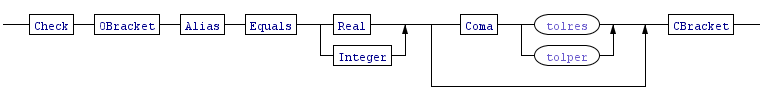
\includegraphics[width=18cm]{contents/images/check.png}
% 	\caption{Diagramme syntaxique du Check}
% \end{figure}
% 		\paragraph{Grammaire de l'Expected Behavior}
% 		Une autre grammaire plus complexe, serait la grammaire des expected Behavior, disponible ci-dessous : 
% \begin{lstlisting}[caption=Grammaire Check, numbers=none, language=C]
% /* Expected Behavior 
%  * Represents what we can meet in an expected Behavior Cell.
%  */
% expectedBehavior: NewLine?((
%                   (If OBracket comparison CBracket Then NewLine? expectedBehavior NewLine?)
%                   (Else NewLine? expectedBehavior NewLine? Endif))
%                   | eval+)
%                   NewLine?;
% \end{lstlisting}
% Le caractère plus \texttt{+} qui n'était pas présent précédemment représente la répétition de l'expression le précédent. Il est ainsi possible d'effectuer n'importe quel grammaire avec ces caractères de base. Comme nous pouvons le voir, la grammaire est récursive. Son diagramme syntaxe est présent figure \ref{fig:diagSynEB}.
% \begin{figure}[H]
% 	\centering
% 		\hspace*{-40px}
% 	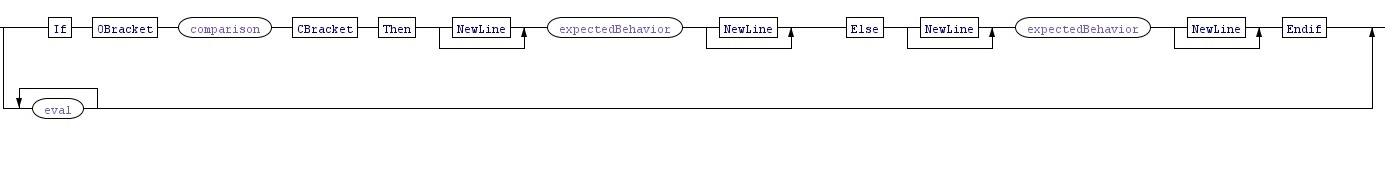
\includegraphics[width=20cm]{contents/images/expectedBehaviorGrammar.jpg}
% 	\caption{Diagramme syntaxique du Check}
% 	\label{fig:diagSynEB}
% \end{figure}
% \begin{remarque}
% Le diagramme devrait contenir des \texttt{Newline} facultatifs au début et à la fin, ceux-ci ont été omis par soucis de lisibilités du diagramme en raison de sa largeur.
% \end{remarque}

% Une fois toutes les grammaires construites avec l'intégralités des n\oe{}uds de l'arbre d'expression, il suffit de générer les fichiers java, et de parcourir l'arbre d'expression.

% 	\subsubsection{La visite de l'arbre d'expression}
% 	Antlr propose plusieurs méthodes afin de reconnaître notre langage, nous avons choisis d'utiliser les \textit{visitors}. Le concept est assez simple : Nous devons hériter d'une classe généré par Antlr, qui est nommée WalkthroughBaseVisitor\footnote{Walkthrough étant le nom du fichier contenant la gramme antlr}, c'est une classe générique nécessitant un type, notre grammaire retournera des String.

% 	Cette classe contient une méthode par token présente dans la grammaire, il est possibles de les surcharger afin d'effectuer nos actions : chacune de ces méthodes ont pour convention de commencer par \texttt{visit} suivis par le nom du token. Ces méthodes sont appelés à chaque fois que nous passons dans ce n\oe{}ud de l'arbre. Celles-ci contiennent en paramètre le n\oe{}ud où l'on se trouve, il est donc possible de chercher des nœuds fils si-besoin, et ensuite d'appeler la suite de l'évaluation de l'arbre. 

% 	J'ai surchargé les méthodes qui était intéressantes ici tel que \texttt{visitCheckFunc(CheckFuncContext ctx)} présenté ci-dessous, le code est commenté afin d'aider à sa compréhension.
% \begin{lstlisting}[language=Java, caption=Surcharge de \texttt{visitCheckFunc}]
% 	@Override
% 	public String visitCheckFunc(CheckFuncContext ctx) {
% 		String aliasName = ctx.getChild(2).toString(); // The alias name to check
% 		if(ctx.getChildCount() > 6) { // If tolerance is present
% 			// It's private method who call the generator, it will be explained after
% 			addCheckParam(aliasName, ctx.getChild(4).toString(), 
% 					(ctx.getChild(6).getChild(0).getText().equals("TOLRES") ? TolType.TOLRES : TolType.TOLPER), 
% 					ctx.getChild(6).getChild(2).getText());
% 		} else {
% 			addCheckParam(aliasName, ctx.getChild(4).toString());
% 		}
% 		// Generator too
% 		aliasReadableRequired.add(new AliasReadable(aliasName));

% 		return super.visitCheckFunc(ctx); // call next node of tree
% 	}
% \end{lstlisting}
% 		\subsubsection{La gestion des exceptions}
% \'Etant donné le temps d'exécution des tests\footnote{Environ une quinzaine d'heures}, il était nécessaire d'effectuer le maximum de vérification avant la phase d'exécution afin de ne pas avoir une erreur qui remonte au bout de plusieurs heures d'exécutions. 

% Pour cela, nous avons utilisés plusieurs stratagèmes, tout d'abord l'utilisation d'un langage fortement typé tel que le Java, à l'opposé du Python utilisé sur la TA3, nous permettait de générer du Java qui en cas d'erreur de type ne compilerait pas\footnote{Comme l'écriture sur un alias en lecture}, mais l'autre approche était l'utilisation des exceptions lors du parsing.

% Une fois le parsing de l'intégralité des variables du Walkthrough, si au moins une ligne n'a pas pu être parsé, une exception est retourné contenant le message de toutes les erreurs trouvés durant ce parsing, toutes les lignes n'ayant pas obtenu d'erreur sont tout de même générés.

% J'ai également mis en place un système de log avec \textit{log4j} qui permet d'afficher proprement des messages de logs et de gérer la sévérité. Si une exception de parsing est renvoyée, celle-ci sera affiché dans la sortie standard, et dans le fichier de log.

% Nous pouvons les dissocier en deux types d'exceptions : les erreurs de syntaxe et les erreurs d'Alias. 
% \paragraph{Erreurs de syntaxe} Ces erreurs sont en partie gérer par Antlr, c'est purement syntaxique tel que l'oubli d'un caractère, cependant les erreurs Antlr n'étant pas clair, j'ai surchargé leurs méthodes d'affichage d'une part, afin d'avoir un affichage comme celui-ci : 
% \begin{lstlisting}[caption=Affichage d'une erreur de syntaxe, numbers=none]
% line 34:10 mismatched input '0' expecting ';'
% HIL_VB  0;
%        ^
% \end{lstlisting}


% \paragraph{Erreurs d'alias} Ces erreurs sont des erreurs sémantiques au niveau des Alias, elles sont regroupés en 3 types différents : 
% \begin{description}
% 	\item[Alias non connu] Cela signifie que l'alias n'est connu nul part, il ne pourra donc pas être résolu lors de l'execution des tests
% 	\item[Alias en lecture seule] L'utilisateur a essayé d'écrire sur un alias en lecture.
% 	\item[Alias en écriture seule] Il n'est pas possible de lire la valeur d'un alias en écriture.\\~
% \end{description}

% \begin{lstlisting}[caption=Affichage d'une erreur d'alias, numbers=none]
% Error: Alias unknown [HL_VSd, Alias, Test]
% Error: Alias not readable [HIL_VS, HIL_VB]
% Error: Alias not writable [HIL_VS_OUT, HIL_VB_OUT]
% \end{lstlisting}
		
% 	\section{Le générateur}
% 	Comme montré dans le schéma \ref{fig:generalDig}, une fois parsé les fichiers doivent être générés. Pour cela, j'ai créé un groupe de classe ayant des services permettant d'ajouter les fonctionnalités à générer : Ajouter un check, ajouter un set, ajouter une action debugger, ajouter les informations des tests, \ldots et lancer la génération du fichier.

% 		\subsection{Génération des tests}
% 		Je dois générer 3types de fichiers : un précondstim, des stimscenario et un GreenTTest pour chaque test. Chacune des classes que je génères hérite de classe présente dans GreenT, respectivement \texttt{PrecondStim}, \texttt{StimScenario} et \texttt{GreenTTest}.

% 		La génération des fichiers possède des points communs en fonction du type de fichier, principalement entre un PrecondStim et un StimScenario, ainsi j'ai conçu un arbre d'héritage assez simple me permettant de factoriser le code : 
% 		\begin{figure}[H]
% 		\centering
% 		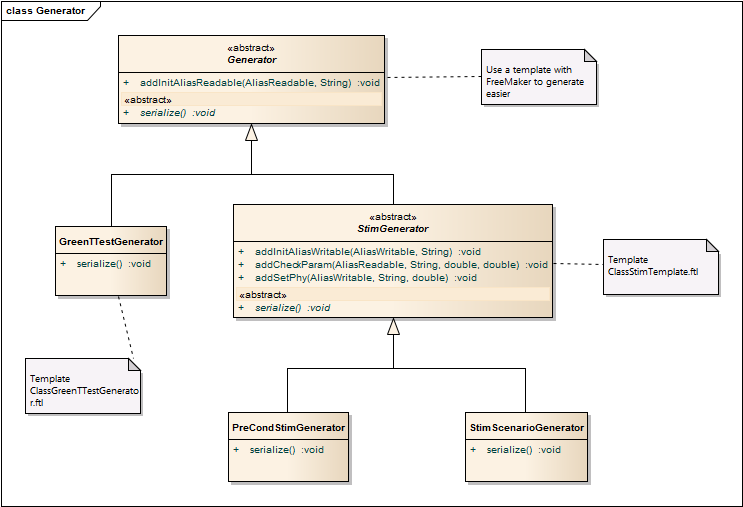
\includegraphics[width=14cm]{contents/images/generatorClass.png}
% 		\caption{Diagramme de classes du générateur}
% 		\end{figure}
% 		La méthode \textit{serialize} écrit le code Java, avant d'appeler cette méthode il est donc nécessaire de << remplir >> l'objet avec les informations nécessaires via les autres méthodes.
		
% 		\subsection{Le moteur de template : freemarker}
% 		\begin{wrapfigure}{l}{3cm}
% 			
\includegraphics[width=3cm]{contents/images/FreeMarker.png}
% 		\end{wrapfigure}
% 		Les classes que je génères ont un gabarit commun, seul l'implémentation des méthodes changent, ainsi plutôt que réécrire systématiquement tout le corps de la classe, il parraissait intéressat d'avoir un moteur de \textit{template}, j'ai choisi FreeMarker.

% 		Ainsi, j'ai un fichier gabarit utilisant son format, avec dedans des appels d'objet, lors de la sérialisation, je fournis à FreeMarker les objets concernés, l'adresse du gabarit et c'est lui qui écrira le fichier \texttt{.java}.
% 		\begin{figure}[H]
% 		\centering
% 		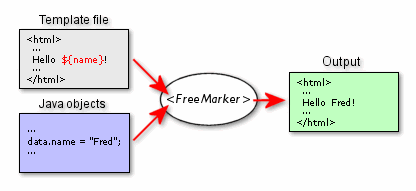
\includegraphics[width=9cm]{contents/images/FreeMarkerSchema.png}
% 		\caption{Schéma de fonctionnement de FreeMarker}
% 		\end{figure}
% 		\begin{remarque}
% 		Cet exemple qui vient du site officiel de FreeMarker utilise des templates HTML, pour ma part j'ai créé des templates Java, mais le principe est le même.
% 		\end{remarque}

% 		Deux fichiers de templates ont été nécessaires : un pour les stim, et un pour le GreenTTest. En effet un preconstim et un stimscenarion n'ont que peu de différence, il était donc possible de les regrouper avec le même template.

% 		Le template des stim contient une liste d'actions à exécuter dans la méthode d'execution, et une liste d'alias nécessaire qui doivent être ajoutés dans une méthode adéquate. \\
% 		Le template des GreenTTest lui contient une méthode permettant de remplir le rapport et une méthode qui créé l'expectedBehavior.
% 		Les deux templates ont également une liste d'import qui est ajoutés automatiquement en début du fichier.

% 		Les deux templates sont disponibles dans l'annexe \ref{annexeTemplate} suivis de deux exemples de fichiers générés disponibles annexe \ref{annexeGeneration}.

% 	\section{L'analyse des traces et la prononciation du verdict}
% 	L'analyse des traces et la prononciation des verdicts, et le c\oe{}ur de GreenT, mais aussi une des parties les plus complexes. Comme expliqué précédemment, lors des stimulations un certain nombre de variables sont enregistrés, ensuite il faut évaluer l'expectedBehavior à chaque instant T de la trace, qui est représenté au format CSV. 

% 	\subsection{Arbre de l'expectedBehavior}
%  	Nous avons choisis de représenter l'expectedBehavior sous la forme d'un arbre d'évaluation, cela nous permettra d'avoir plus de souplesse, en pouvant donner un verdict à une partie de l'arbre.

%  	Ainsi, chaque conditions de l'expected behavior peut être transformé en une implication logique, plusieurs eval à la suite correspondent à un et logique de chacune des conditions des evals, et enfin, un else implique d'avoir eu la négation de la condition précédente. Figure \ref{fig:diagLogique}, nous pouvons voir un exemple d'expectedBehavior et sa transformation en arbre.

%  	\begin{figure}[H]
%  		\centering
%  		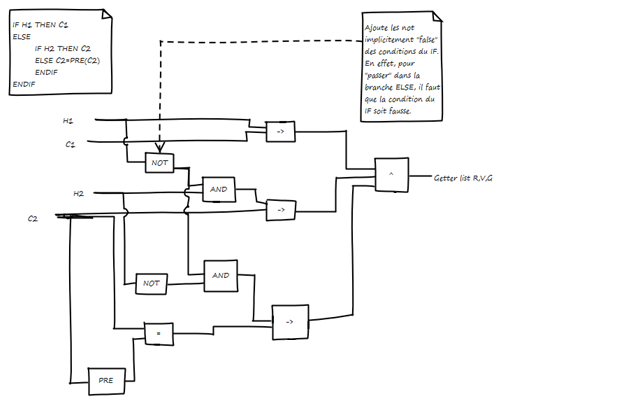
\includegraphics[width=18cm]{contents/images/diagLogique.png}
%  		\caption{Transformation d'une expectedBehavior en arbre logique}
%  		\label{fig:diagLogique}
%  	\end{figure}

% L'expected Behavior contiendra des variables, celles-ci pourront être modifier à tout moment ce qui relancera son évaluation, elle sera notifié de cette modification à l'aide du design pattern \textit{Observer}. Une variable peut être spécifique en fonction du type de la variable, ceci afin d'aider les conversions.

% Une expectedBehavior peut recevoir 3 états différents à l'issue de l'évaluation de la trace : 
% \begin{description}
% 	\item[Rouge] Au moins un eval à renvoyé faux
% 	\item[Gris] Aucun eval n'a renvoyé faux, mais au moins une branche n'a pas été testé
% 	\item[Vert] Toutes les branches ont été testé, et tous les eval ont renvoyés vrais.
% \end{description}

% 	\subsection{Analyse de la trace}
% 	Le fichier de trace au format CSV va être transformé en une Map ayant pour clé le timestamp et pour valeur la liste des variables ayant subis une modification, ainsi nous allons avoir une boucle itérant sur cette Map qui à chaque itération modifiera les variables nécessaire, lors de cette modification une notification va être envoyé à l'expectedBehavior qui relancera l'évaluation de la trace, le \texttt{TraceAnalyzer} stockera ce résultat dans le rapport. 

% 	De cette manière, il sera possible d'analyser l'expected Behavior à tout instant T de la trace.
%  	\begin{figure}[H]
%  		\centering
%  		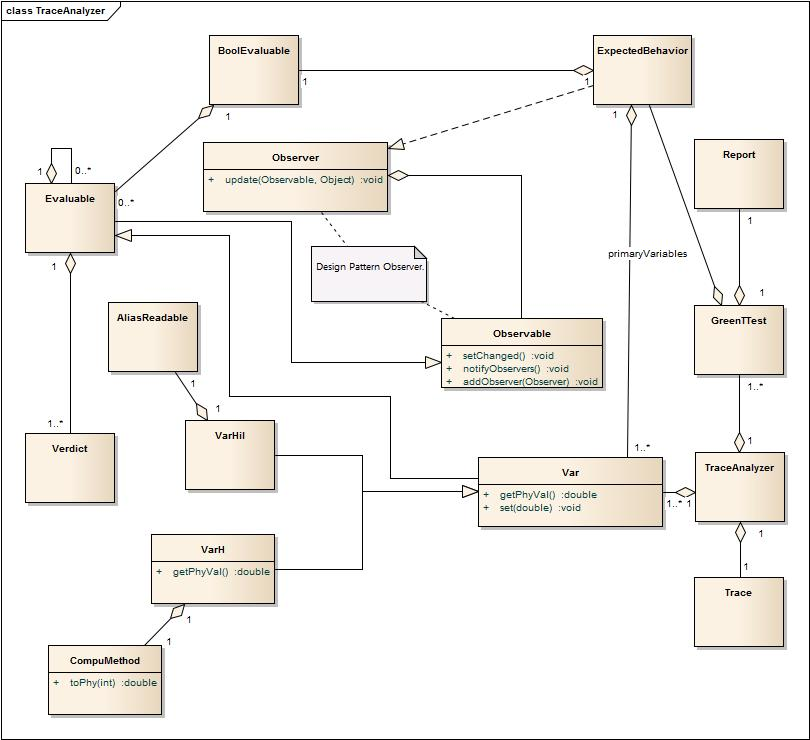
\includegraphics[width=15.5cm]{contents/images/TraceAnalyzer.jpg}
%  		\caption{Diagramme de classe de l'analyse de trace}
%  		\label{fig:diagLogique}
%  	\end{figure}
%  	Le n\oe{}ud racine de l'arbre d'expression sera un \texttt{BoolEvaluable} possédant un verdict(Rouge, Gris, Vert), et chaque n\oe{}ud de l'arbre et donc les \texttt{Variables} seront des \texttt{Evaluables}.
% 	\subsection{Prononciation du verdict}
% 	Chaque n\oe{}ud de l'arbre d'expression est susceptible d'avoir son propre verdict : ceci afin d'avoir plus de souplesse. Dans notre cas, seul les implications correspondant à une branche de \texttt{if...else} possèdera un verdict.
